\chapter{LEA: Implementation in Little-Endian}
\section{Specification}

\begin{table}[h]
	\centering
	\caption{Specification Comparison between AES and LEA Block Ciphers}
	\begin{tabular*}{\textwidth}{@{\extracolsep{\fill}}>{\bfseries}l||cc}
		\toprule
		Specification & \textcolor{red}{\bf AES} & \textcolor{blue}{\bf LEA} \\
		\midrule
		Block Size (bits) & 128 & 128 \\
		Key Size (bits) & 128/192/256 & 128/192/256 \\
		Structure & \textcolor{red}{S}ubstitution-\textcolor{red}{P}ermutation \textcolor{red}{N}etwork & \textcolor{blue}{G}eneralized \textcolor{blue}{F}eistel \textcolor{blue}{N}etwork \\
		Rounds & 10/12/14 (depends on key size) & 24/28/32 (depends on key size) \\
		Design Year & 1998 & 2013 \\
		\bottomrule
	\end{tabular*}
\end{table}

\begin{table}[h!]\centering\renewcommand{\arraystretch}{1.25} % Increase row height by 1.5 times
	\caption{Parameters of the Block Cipher LEA (1-word = 32-bit)}
	\begin{tabular*}{\textwidth}{@{\extracolsep{\fill}}>{\bfseries}c||cccccc}
		\toprule[1.2pt]
		\multirow{3}{*}{Algorithms} & Block & Key & Number of & Round-Key & Number of & Total Size of\\
		& Size & Length & Rounds &  Length & Round-Keys & Round-Keys \\
		& ($N_b$-byte) & ($N_k$-byte) & ($N_r$)& (byte) & ($N_r+1$)& ($N_b(N_r+1)$)\\
		\hline\hline
		LEA-128 & 16(4-word) & 16(4-word) & 24 & 24 & 11 & 44 (176-byte) \\
		LEA-192 & 16(4-word) & 24(6-word) & 28 & 24 & 13 & 52 (208-byte) \\
		LEA-256 & 16(4-word) & 32(8-word) & 32 & 24 & 15 & 60 (240-byte) \\
		\bottomrule[1.2pt]
	\end{tabular*}
\end{table}

\section{State Representation}

Let $\state[0],\state[1], \dots$ be representation of arrays of bytes.
Note that \[
\state[i]:=\set{input_{8i},input_{8i+1},\dots,input_{8i+7}}\in\F_{2^8}
\] for $input_{i}\in\F_2$. For example, $\state[0]=\set{input_0,input_1,\dots,input_7}$.

The 128-bit plaintext $P$ of LEA is represented as an array of four 32-bit words $P[0],P[1],P[2]$ and $P[3]$. Then \[
P[i] = \state[4i+3]\adjacent\state[4i+2]\adjacent\state[4i+1]\adjacent\state[4i]\quad\text{for}\quad 0\leq i\leq 3.
\] Here, $P[i]\in\F_{2^{32=8\cdot 4}}$The key $K$ of LEA is also represented as the same way.

\newpage
\begin{table}[h!]\centering\renewcommand{\arraystretch}{1.25} % Increase row height by 1.5 times
	\caption{Representations for words, bytes, and bits}
	\begin{tabular}{@{\extracolsep{\fill}}>{\bfseries}l||c|c|c|c|c|c|c|c|c|c|c|c}
		\toprule[1.2pt]
		Input Bit Sequence & \cellcolor{red!20}24 & \cellcolor{red!20}$\cdots$ & \cellcolor{red!20}31 & \cellcolor{green!20}16 & \cellcolor{green!20}$\cdots$ & \cellcolor{green!20}23 & \cellcolor{blue!20}8 & \cellcolor{blue!20}$\cdots$ & \cellcolor{blue!20}15 & \cellcolor{orange!20}0 & \cellcolor{orange!20}$\cdots$ & \cellcolor{orange!20}7\\
		\hline
		Word Number & \multicolumn{12}{c}{0}\\
		\hline
		Byte Number & \multicolumn{3}{c|}{3} & \multicolumn{3}{c|}{2} & \multicolumn{3}{c|}{1} & \multicolumn{3}{c}{0}\\
		\hline
		Bit Numbers in Word & 31 & \multicolumn{10}{|c|}{$\cdots$} & 1\\
		\bottomrule[1.2pt]
	\end{tabular}
\end{table}

\begin{example}
\ \begin{table}[h!]\centering\renewcommand{\arraystretch}{1.25} % Increase row height by 1.5 times
	\begin{tabular}{@{\extracolsep{\fill}}>{\bfseries}l||c|c|c|c|c|c|c|c|c|c|c|c}
		\toprule[1.2pt]
		128-bit Input String & \multicolumn{12}{c}{\texttt{0x0f1e2d3c4b5a69788796a5b4c3d2e1f0}} \\
		\hline
		\multirow{2}{*}{Split into Words} & \multicolumn{3}{c|}{0x0f1e2d3c} & \multicolumn{3}{c|}{0x4b5a6978} & \multicolumn{3}{c|}{0x8796a5b4} & \multicolumn{3}{c}{0xc3d2e1f0} \\
		& \multicolumn{3}{c|}{$P[0]$} & \multicolumn{3}{c|}{$P[1]$} & \multicolumn{3}{c|}{$P[2]$} & \multicolumn{3}{c}{$P[3]$}\\
		\hline
		$P[0]$ (Word) & \multicolumn{12}{c}{0x0f1e2d3c} \\
		\hline
		$P[0]$ (Bit) & \multicolumn{12}{c}{0b 0000:1111:0001:1110:0010:1101:0011:1010} \\
		\hline
		\multirow{2}{*}{Split into Bytes} & \multicolumn{3}{c|}{0x0f} & \multicolumn{3}{c|}{0x1e} & \multicolumn{3}{c|}{0x2d} & \multicolumn{3}{c}{0x3c} \\
		& \multicolumn{3}{c|}{$\state[3]$} & \multicolumn{3}{c|}{$\state[2]$} & \multicolumn{3}{c|}{$\state[1]$} & \multicolumn{3}{c}{$\state[0]$}\\
		\hline
		$\state[0]$ (Byte) & \multicolumn{12}{c}{0x3c} \\
		\hline
		\multirow{2}{*}{Split into Bits} & \multicolumn{3}{c|}{1111:0000} & \multicolumn{3}{c|}{-} & \multicolumn{3}{c|}{-} & \multicolumn{3}{c}{-} \\
		& \cellcolor{red!20}24 & \cellcolor{red!20}$\cdots$ & \cellcolor{red!20}31 & \cellcolor{green!20}16 & \cellcolor{green!20}$\cdots$ & \cellcolor{green!20}23 & \cellcolor{blue!20}8 & \cellcolor{blue!20}$\cdots$ & \cellcolor{blue!20}15 & \cellcolor{orange!20}0 & \cellcolor{orange!20}$\cdots$ & \cellcolor{orange!20}7\\
		\bottomrule[1.2pt]
	\end{tabular}
\end{table}
\end{example}

\begin{lstlisting}[style=C]
const char* inputString = "0f1e2d3c4b5a69788796a5b4c3d2e1f0";
u32 key[4];
stringToWordArray(inputString, key);

/*
(gdb) x/32xb key
0x7fffffffd9c0:	0x3c	0x2d	0x1e	0x0f
				0x78	0x69	0x5a	0x4b
0x7fffffffd9c8:	0xb4	0xa5	0x96	0x87
				0xf0	0xe1	0xd2	0xc3
0x7fffffffd9d0:	0x01	0x00	0x00	0x00
				0x00	0x00	0x00	0x00
0x7fffffffd9d8:	0xf6	0x75	0xae	0x03
				0x01	0x00	0x00	0x00
*/
\end{lstlisting}

\section{Key Schedule}

$$
\text{KeySchedule}^{\enc}_{128}:\binaryfield^{128=8\cdot 16}\to\binaryfield^{4608=192\cdot 24}
$$

$$
\text{KeySchedule}^{\enc}_{192}:\binaryfield^{192=8\cdot 24}\to\binaryfield^{5376=192\cdot 28}
$$

$$
\text{KeySchedule}^{\enc}_{256}:\binaryfield^{256=8\cdot 32}\to\binaryfield^{6144=192\cdot 24}
$$

\subsection{Round Constant}
The constant $\delta[i]\in\F_{2^{32}}$ ($i\in\set{1,\dots,7}$) is as follows:
\begin{table}[h!]\centering\renewcommand{\arraystretch}{1.25} % Increase row height by 1.5 times
	\begin{tabular}{c|lc}
		$i$ & $\delta[i]$ & value\\
		\midrule
		0 & $\delta[0]$ & \texttt{0xc3efe9db}\\
		1 & $\delta[1]$ & \texttt{0x44626b02}\\
		2 & $\delta[2]$ & \texttt{0x79e27c8a}\\
		3 & $\delta[3]$ & \texttt{0x78df30ec}\\
		4 & $\delta[4]$ & \texttt{0x715ea49e}\\
		5 & $\delta[5]$ & \texttt{0xc785da0a}\\
		6 & $\delta[6]$ & \texttt{0xe04ef22a}\\
		7 & $\delta[7]$ & \texttt{0xe5c40957}
	\end{tabular}
\end{table}

\subsection{Rotation Function}

\begin{algorithm}[H]
	\caption{Rotation to Left and Right}
	\SetKwFunction{FRotL}{RotL}
	\SetKwFunction{FRotR}{RotR}
	\Comment{$\texttt{RotL}:\binaryfield^{32}\times\binaryfield^{32}\to\binaryfield^{32}$}
	\Fn{\FRotL{\textnormal{value, shift}}}{
		\KwRet{$(\textnormal{value} \ll \textnormal{shift}) \;|\; (\textnormal{value} \gg (32 -  \textnormal{shift}))$}\;
	}
	\BlankLine
	\Comment{$\texttt{RotR}:\binaryfield^{32}\times\binaryfield^{32}\to\binaryfield^{32}$}
	\Fn{\FRotR{\textnormal{value, shift}}}{
		\KwRet{$(\textnormal{value} \gg \textnormal{shift}) \;|\; (\textnormal{value} \ll (32 - \textnormal{shift}))$}\;
	}
\end{algorithm}

\subsection{Encryption Key Schedule of LEA-128}

\begin{algorithm}[H]
	\caption{Encryption Key Schedule (LEA-128)}
	\DontPrintSemicolon
	\KwIn{User-key \( \uk = \uk[0]\adjacent\uk[1]\adjacent\uk[2]\adjacent\uk[3] \) \( (\uk[i] \in \binaryfield^{32}) \)}
	\KwOut{Encryption Round-keys \( \{\rk^{\enc}_i\}_{i=0}^{23} \) \( (\rk^{\enc}_i \in \binaryfield^{192}) \)}
	\Comment{$\uk\in\binaryfield^{128}$ is 16-byte and $\set{\rk^{\enc}_i}_{i=0}^{23}\in\binaryfield^{4608}$ is 576-byte}
	\BlankLine
	\For{\( i = 0 \) \KwTo \( 3 \)}{
		$T[i]=\uk[i]$\tcp*{$T=T[0]\adjacent\cdots\adjacent T[3]\in\binaryfield^{128=32*4}$}
	}
%	$T=T[3]\adjacent T[2]\adjacent T[1]\adjacent T[0]\gets\uk$\tcp*{$T\in\binaryfield^{128=32*4}$}
	\For{\( i = 0 \) \KwTo \( 23 \)}{
		$T[0]\gets\RotL(T[0]\boxplus\RotL(\delta[i\bmod 4],i+0),1)$\tcp*{$T[i]\in\binaryfield^{32}$}
		$T[1]\gets\RotL(T[1]\boxplus\RotL(\delta[i\bmod 4],i+1),3)$\;
		$T[2]\gets\RotL(T[2]\boxplus\RotL(\delta[i\bmod 4],i+2),6)$\;
		$T[3]\gets\RotL(T[3]\boxplus\RotL(\delta[i\bmod 4],i+3),11)$\;
		$\rk^{\enc}_i\gets T[0]\adjacent T[1]\adjacent T[2]\adjacent T[1]\adjacent T[3]\adjacent T[1]$\tcp*{$\rk^{\enc}_i\in\binaryfield^{196=32*6}$}
	}
	\Return $\set{\rk^{\enc}_i}_{i=0}^{23}$\;
\end{algorithm}

%\subsection{Key Schedule 192}

%\subsection{Key Schedule 256}

\newpage
\section{Encryption of LEA-128}

\begin{algorithm}[H]
	\caption{Encryption of LEA-128}
	\DontPrintSemicolon
	\KwIn{block $\mathsf{src}=\src[0]\adjacent\src[1]\adjacent\src[2]\adjacent\src[3] \in \binaryfield^{128=32*4}$ and $\{\rk^{\enc}_i\}_{i=0}^{N_r-1=23}$}
	\KwOut{block $\mathsf{dst}=\dsc[0]\adjacent\dsc[1]\adjacent\dsc[2]\adjacent\dsc[3] \in \binaryfield^{128=32*4}$}
	\BlankLine
	$t_0=t[0]\adjacent t[1]\adjacent t[2]\adjacent t[3]\gets\src$\;
	\For{$i=0$ \KwTo $23$}{
		$tmp\gets t[0]$\;
		$t_{i+1}[0]\gets\RotL(\mathcolorbox{cyan!20}{t_i[0]\oplus\rk^{\enc}_i[0]}\mathcolorbox{red!20}{\boxplus}\mathcolorbox{green!20}{(t_{i}[1]\oplus\rk^{\enc}_i[1])}, 9)$\;
		$t_{i+1}[1]\gets\RotR(\mathcolorbox{orange!20}{t_i[1]\oplus\rk^{\enc}_i[2]}\mathcolorbox{red!20}{\boxplus}\mathcolorbox{blue!20}{(t_{i}[2]\oplus\rk^{\enc}_i[3])}, 5)$\;
		$t_{i+1}[2]\gets\RotR(\mathcolorbox{yellow!20}{t_i[2]\oplus\rk^{\enc}_i[4]}\mathcolorbox{red!20}{\boxplus}\mathcolorbox{violet!20}{(t_{i}[3]\oplus\rk^{\enc}_i[5])}, 3)$\;
		$t_{i+1}[3]\gets tmp$\;
	}
	\Return{$\mathsf{dst}\gets t_{N_r}$}\;
\end{algorithm}


\begin{center}
\tikzset{every picture/.style={line width=0.75pt}} %set default line width to 0.75pt        
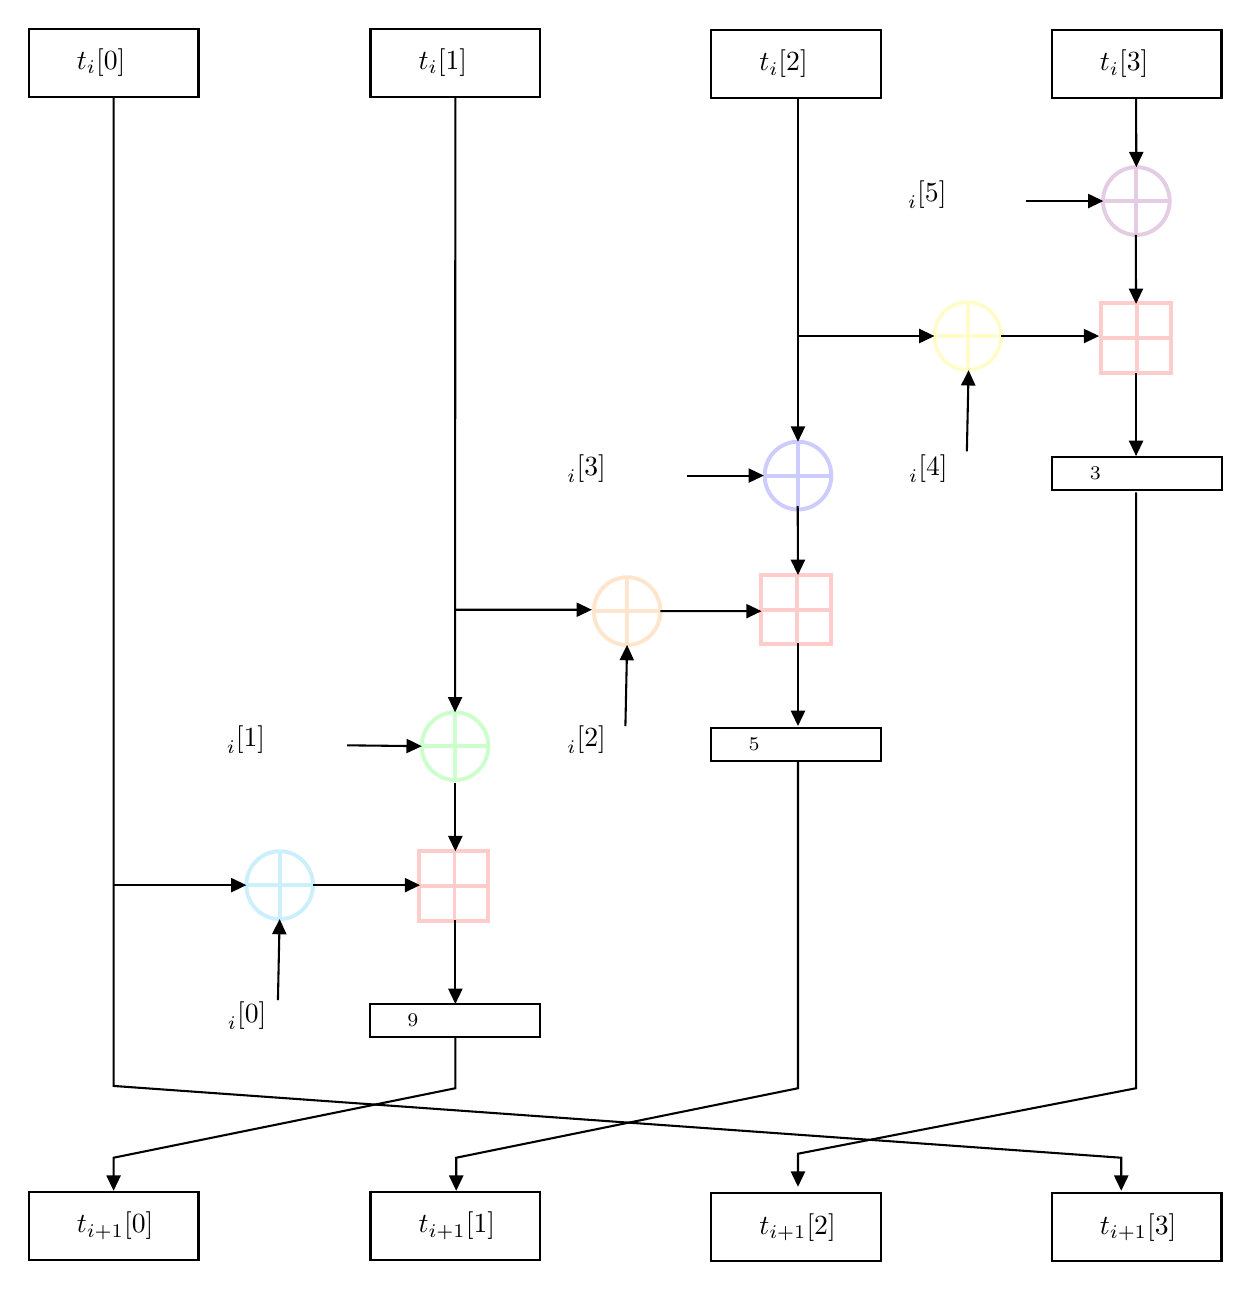
\begin{tikzpicture}[x=0.65pt,y=0.65pt,yscale=-.95,xscale=.95]
	%uncomment if require: \path (0,761); %set diagram left start at 0, and has height of 761
	
	%Shape: Rectangle [id:dp09649710923858557] 
	\draw   (1.33,19.67) -- (100.67,19.67) -- (100.67,59.68) -- (1.33,59.68) -- cycle ;
	%Shape: Rectangle [id:dp09856796445221394] 
	\draw   (201.33,19.67) -- (300.67,19.67) -- (300.67,59.68) -- (201.33,59.68) -- cycle ;
	%Shape: Rectangle [id:dp8562072452851615] 
	\draw   (400.67,20.33) -- (500,20.33) -- (500,60.34) -- (400.67,60.34) -- cycle ;
	%Shape: Rectangle [id:dp2992411273709372] 
	\draw   (600,20.33) -- (699.33,20.33) -- (699.33,60.34) -- (600,60.34) -- cycle ;
	%Flowchart: Or [id:dp009962572646309509] 
	\draw[violet!20, line width=.5mm]   (630,120.51) .. controls (630,109.55) and (638.73,100.67) .. (649.5,100.67) .. controls (660.27,100.67) and (669,109.55) .. (669,120.51) .. controls (669,131.46) and (660.27,140.34) .. (649.5,140.34) .. controls (638.73,140.34) and (630,131.46) .. (630,120.51) -- cycle ; \draw[violet!20, line width=.5mm]   (630,120.51) -- (669,120.51) ; \draw[violet!20, line width=.5mm]   (649.5,100.67) -- (649.5,140.34) ;
	\draw[red!20, line width=.5mm]   (630,200.83) -- (669.67,200.83)(649.83,180.67) -- (649.83,221) ;
	%Shape: Square [id:dp09147464413397532] 
	\draw[red!20, line width=.5mm]   (629,180.33) -- (669.67,180.33) -- (669.67,221) -- (629,221) -- cycle ;
	
	%Shape: Rectangle [id:dp09967017747119322] 
	\draw  (600.33,270.34) -- (699.67,270.34) -- (699.67,289.68) -- (600.33,289.68) -- cycle ;
	
	%Flowchart: Or [id:dp36172575810966023] 
	\draw[yellow!20, line width=.5mm]   (531.33,199.51) .. controls (531.33,188.55) and (540.06,179.67) .. (550.83,179.67) .. controls (561.6,179.67) and (570.33,188.55) .. (570.33,199.51) .. controls (570.33,210.46) and (561.6,219.34) .. (550.83,219.34) .. controls (540.06,219.34) and (531.33,210.46) .. (531.33,199.51) -- cycle ; \draw[yellow!20, line width=.5mm]   (531.33,199.51) -- (570.33,199.51) ; \draw[yellow!20, line width=.5mm]   (550.83,179.67) -- (550.83,219.34) ;
	%Flowchart: Or [id:dp6962690504121853] 
	\draw[blue!20, line width=.5mm]   (432,281.17) .. controls (432,270.22) and (440.73,261.33) .. (451.5,261.33) .. controls (462.27,261.33) and (471,270.22) .. (471,281.17) .. controls (471,292.13) and (462.27,301.01) .. (451.5,301.01) .. controls (440.73,301.01) and (432,292.13) .. (432,281.17) -- cycle ; \draw[blue!20, line width=.5mm]   (432,281.17) -- (471,281.17) ; \draw[blue!20, line width=.5mm]   (451.5,261.33) -- (451.5,301.01) ;
	\draw[red!20, line width=.5mm]   (431,359.83) -- (470.67,359.83)(450.83,339.67) -- (450.83,380) ;
	%Shape: Square [id:dp6617373124522021] 
	\draw[red!20, line width=.5mm]   (430,339.33) -- (470.67,339.33) -- (470.67,380) -- (430,380) -- cycle ;
	
	%Shape: Rectangle [id:dp7113161895052367] 
	\draw   (400.67,429.01) -- (500,429.01) -- (500,448.34) -- (400.67,448.34) -- cycle ;
	
	%Flowchart: Or [id:dp41104666078269214] 
	\draw[orange!20, line width=.5mm]   (332,360.49) .. controls (332,349.54) and (340.73,340.66) .. (351.5,340.66) .. controls (362.27,340.66) and (371,349.54) .. (371,360.49) .. controls (371,371.45) and (362.27,380.33) .. (351.5,380.33) .. controls (340.73,380.33) and (332,371.45) .. (332,360.49) -- cycle ; \draw[orange!20, line width=.5mm]   (332,360.49) -- (371,360.49) ; \draw[orange!20, line width=.5mm]   (351.5,340.66) -- (351.5,380.33) ;
	%Flowchart: Or [id:dp0838978643716497] 
	\draw[green!20, line width=.5mm]   (231.33,439.52) .. controls (231.33,428.56) and (240.06,419.68) .. (250.83,419.68) .. controls (261.6,419.68) and (270.33,428.56) .. (270.33,439.52) .. controls (270.33,450.47) and (261.6,459.35) .. (250.83,459.35) .. controls (240.06,459.35) and (231.33,450.47) .. (231.33,439.52) -- cycle ; \draw[green!20, line width=.5mm]   (231.33,439.52) -- (270.33,439.52) ; \draw[green!20, line width=.5mm]   (250.83,419.68) -- (250.83,459.35) ;
	\draw[red!20, line width=.5mm]   (230.67,521.5) -- (270.33,521.5)(250.5,501.33) -- (250.5,541.67) ;
	%Shape: Square [id:dp86851145355007] 
	\draw[red!20, line width=.5mm]   (229.67,501) -- (270.33,501) -- (270.33,541.67) -- (229.67,541.67) -- cycle ;
	
	%Shape: Rectangle [id:dp7193799781611718] 
	\draw   (201,590.34) -- (300.33,590.34) -- (300.33,609.68) -- (201,609.68) -- cycle ;
	
	%Flowchart: Or [id:dp7288306958593842] 
	\draw[cyan!20, line width=.5mm]   (128.67,520.84) .. controls (128.67,509.88) and (137.4,501) .. (148.17,501) .. controls (158.94,501) and (167.67,509.88) .. (167.67,520.84) .. controls (167.67,531.8) and (158.94,540.68) .. (148.17,540.68) .. controls (137.4,540.68) and (128.67,531.8) .. (128.67,520.84) -- cycle ; \draw[cyan!20, line width=.5mm]   (128.67,520.84) -- (167.67,520.84) ; \draw[cyan!20, line width=.5mm]   (148.17,501) -- (148.17,540.68) ;
	%Shape: Rectangle [id:dp8154253641610185] 
	\draw   (1.33,700.33) -- (100.67,700.33) -- (100.67,740.34) -- (1.33,740.34) -- cycle ;
	%Shape: Rectangle [id:dp17512457192518172] 
	\draw   (201.33,700.33) -- (300.67,700.33) -- (300.67,740.34) -- (201.33,740.34) -- cycle ;
	%Shape: Rectangle [id:dp9808199440526231] 
	\draw   (400.67,701) -- (500,701) -- (500,741.01) -- (400.67,741.01) -- cycle ;
	%Shape: Rectangle [id:dp30331440009031585] 
	\draw   (600,701) -- (699.33,701) -- (699.33,741.01) -- (600,741.01) -- cycle ;
	%Straight Lines [id:da9905277442894351] 
	\draw    (649.33,60.34) -- (649.49,97.67) ;
	\draw [shift={(649.5,100.67)}, rotate = 269.76] [fill={rgb, 255:red, 0; green, 0; blue, 0 }  ][line width=0.08]  [draw opacity=0] (8.93,-4.29) -- (0,0) -- (8.93,4.29) -- cycle    ;
	%Straight Lines [id:da9180893972119539] 
	\draw    (649.17,140.34) -- (649.32,177.67) ;
	\draw [shift={(649.33,180.67)}, rotate = 269.76] [fill={rgb, 255:red, 0; green, 0; blue, 0 }  ][line width=0.08]  [draw opacity=0] (8.93,-4.29) -- (0,0) -- (8.93,4.29) -- cycle    ;
	%Straight Lines [id:da5776414493110817] 
	\draw    (649.33,221.01) -- (649.33,266.69) ;
	\draw [shift={(649.33,269.69)}, rotate = 270] [fill={rgb, 255:red, 0; green, 0; blue, 0 }  ][line width=0.08]  [draw opacity=0] (8.93,-4.29) -- (0,0) -- (8.93,4.29) -- cycle    ;
	%Straight Lines [id:da3007073804050684] 
	\draw    (451.5,60.34) -- (451.5,258.33) ;
	\draw [shift={(451.5,261.33)}, rotate = 270] [fill={rgb, 255:red, 0; green, 0; blue, 0 }  ][line width=0.08]  [draw opacity=0] (8.93,-4.29) -- (0,0) -- (8.93,4.29) -- cycle    ;
	%Straight Lines [id:da3894439892001873] 
	\draw    (451.5,199.51) -- (528.33,199.51) ;
	\draw [shift={(531.33,199.51)}, rotate = 180] [fill={rgb, 255:red, 0; green, 0; blue, 0 }  ][line width=0.08]  [draw opacity=0] (8.93,-4.29) -- (0,0) -- (8.93,4.29) -- cycle    ;
	%Straight Lines [id:da7364555228497087] 
	\draw    (570.33,199.51) -- (624.67,199.51) ;
	\draw [shift={(627.67,199.51)}, rotate = 180] [fill={rgb, 255:red, 0; green, 0; blue, 0 }  ][line width=0.08]  [draw opacity=0] (8.93,-4.29) -- (0,0) -- (8.93,4.29) -- cycle    ;
	%Straight Lines [id:da31496740554012526] 
	\draw    (585,120.51) -- (627.17,120.51) ;
	\draw [shift={(630.17,120.51)}, rotate = 180] [fill={rgb, 255:red, 0; green, 0; blue, 0 }  ][line width=0.08]  [draw opacity=0] (8.93,-4.29) -- (0,0) -- (8.93,4.29) -- cycle    ;
	%Straight Lines [id:da8515918812814016] 
	\draw    (550.33,267.02) -- (551.27,222.5) ;
	\draw [shift={(551.33,219.51)}, rotate = 91.21] [fill={rgb, 255:red, 0; green, 0; blue, 0 }  ][line width=0.08]  [draw opacity=0] (8.93,-4.29) -- (0,0) -- (8.93,4.29) -- cycle    ;
	%Straight Lines [id:da4312154735895857] 
	\draw    (386.33,281.17) -- (428.5,281.17) ;
	\draw [shift={(431.5,281.17)}, rotate = 180] [fill={rgb, 255:red, 0; green, 0; blue, 0 }  ][line width=0.08]  [draw opacity=0] (8.93,-4.29) -- (0,0) -- (8.93,4.29) -- cycle    ;
	%Straight Lines [id:da16609584587582016] 
	\draw    (451.33,299.01) -- (451.49,336.33) ;
	\draw [shift={(451.5,339.33)}, rotate = 269.76] [fill={rgb, 255:red, 0; green, 0; blue, 0 }  ][line width=0.08]  [draw opacity=0] (8.93,-4.29) -- (0,0) -- (8.93,4.29) -- cycle    ;
	%Straight Lines [id:da08792297598453813] 
	\draw    (451.5,379.35) -- (451.5,424.69) ;
	\draw [shift={(451.5,427.69)}, rotate = 270] [fill={rgb, 255:red, 0; green, 0; blue, 0 }  ][line width=0.08]  [draw opacity=0] (8.93,-4.29) -- (0,0) -- (8.93,4.29) -- cycle    ;
	%Straight Lines [id:da9661600748076484] 
	\draw    (251,60.34) -- (250.83,416.68) ;
	\draw [shift={(250.83,419.68)}, rotate = 270.03] [fill={rgb, 255:red, 0; green, 0; blue, 0 }  ][line width=0.08]  [draw opacity=0] (8.93,-4.29) -- (0,0) -- (8.93,4.29) -- cycle    ;
	%Straight Lines [id:da21962023006454734] 
	\draw    (51,60.34) -- (51,638.35) -- (640.67,680.35) -- (640.67,696.67) ;
	\draw [shift={(640.67,699.67)}, rotate = 270] [fill={rgb, 255:red, 0; green, 0; blue, 0 }  ][line width=0.08]  [draw opacity=0] (8.93,-4.29) -- (0,0) -- (8.93,4.29) -- cycle    ;
	%Straight Lines [id:da10170207411003251] 
	\draw    (187.67,439.02) -- (228.33,439.48) ;
	\draw [shift={(231.33,439.52)}, rotate = 180.65] [fill={rgb, 255:red, 0; green, 0; blue, 0 }  ][line width=0.08]  [draw opacity=0] (8.93,-4.29) -- (0,0) -- (8.93,4.29) -- cycle    ;
	%Straight Lines [id:da7472855698291854] 
	\draw    (251,461) -- (251,498) ;
	\draw [shift={(251,501)}, rotate = 270] [fill={rgb, 255:red, 0; green, 0; blue, 0 }  ][line width=0.08]  [draw opacity=0] (8.93,-4.29) -- (0,0) -- (8.93,4.29) -- cycle    ;
	%Straight Lines [id:da4315863901810195] 
	\draw    (371,360.49) -- (427.17,360.5) ;
	\draw [shift={(430.17,360.51)}, rotate = 180.01] [fill={rgb, 255:red, 0; green, 0; blue, 0 }  ][line width=0.08]  [draw opacity=0] (8.93,-4.29) -- (0,0) -- (8.93,4.29) -- cycle    ;
	%Straight Lines [id:da8749159261902415] 
	\draw    (251,359.67) -- (327.83,359.68) ;
	\draw [shift={(330.83,359.68)}, rotate = 180.01] [fill={rgb, 255:red, 0; green, 0; blue, 0 }  ][line width=0.08]  [draw opacity=0] (8.93,-4.29) -- (0,0) -- (8.93,4.29) -- cycle    ;
	%Straight Lines [id:da8945918947420974] 
	\draw    (350.5,427.85) -- (351.44,383.33) ;
	\draw [shift={(351.5,380.33)}, rotate = 91.21] [fill={rgb, 255:red, 0; green, 0; blue, 0 }  ][line width=0.08]  [draw opacity=0] (8.93,-4.29) -- (0,0) -- (8.93,4.29) -- cycle    ;
	%Straight Lines [id:da951987715770007] 
	\draw    (147.17,588.19) -- (148.1,543.68) ;
	\draw [shift={(148.17,540.68)}, rotate = 91.21] [fill={rgb, 255:red, 0; green, 0; blue, 0 }  ][line width=0.08]  [draw opacity=0] (8.93,-4.29) -- (0,0) -- (8.93,4.29) -- cycle    ;
	%Straight Lines [id:da3034859131323091] 
	\draw    (167.67,520.84) -- (227.33,520.84) ;
	\draw [shift={(230.33,520.84)}, rotate = 180] [fill={rgb, 255:red, 0; green, 0; blue, 0 }  ][line width=0.08]  [draw opacity=0] (8.93,-4.29) -- (0,0) -- (8.93,4.29) -- cycle    ;
	%Straight Lines [id:da4266925461976472] 
	\draw    (251,541) -- (251,587.35) ;
	\draw [shift={(251,590.35)}, rotate = 270] [fill={rgb, 255:red, 0; green, 0; blue, 0 }  ][line width=0.08]  [draw opacity=0] (8.93,-4.29) -- (0,0) -- (8.93,4.29) -- cycle    ;
	%Straight Lines [id:da6182103187618337] 
	\draw    (51,520.84) -- (125.67,520.84) ;
	\draw [shift={(128.67,520.84)}, rotate = 180] [fill={rgb, 255:red, 0; green, 0; blue, 0 }  ][line width=0.08]  [draw opacity=0] (8.93,-4.29) -- (0,0) -- (8.93,4.29) -- cycle    ;
	%Straight Lines [id:da19329858602080163] 
	\draw    (251,609.68) -- (251,639.69) -- (51,680.35) -- (51,696.67) ;
	\draw [shift={(51,699.67)}, rotate = 270] [fill={rgb, 255:red, 0; green, 0; blue, 0 }  ][line width=0.08]  [draw opacity=0] (8.93,-4.29) -- (0,0) -- (8.93,4.29) -- cycle    ;
	%Straight Lines [id:da5896013822532502] 
	\draw    (451.5,448.34) -- (451.5,639.69) -- (251.5,680.35) -- (251.5,696.67) ;
	\draw [shift={(251.5,699.67)}, rotate = 270] [fill={rgb, 255:red, 0; green, 0; blue, 0 }  ][line width=0.08]  [draw opacity=0] (8.93,-4.29) -- (0,0) -- (8.93,4.29) -- cycle    ;
	%Straight Lines [id:da43315106333049536] 
	\draw    (649.33,291.02) -- (649.33,639.69) -- (451.5,678.01) -- (451.5,694.32) ;
	\draw [shift={(451.5,697.32)}, rotate = 270] [fill={rgb, 255:red, 0; green, 0; blue, 0 }  ][line width=0.08]  [draw opacity=0] (8.93,-4.29) -- (0,0) -- (8.93,4.29) -- cycle    ;
	
	% Text Node
	\draw (51,39.67) node   [align=left] {\begin{minipage}[lt]{26.52pt}\setlength\topsep{0pt}
			$\displaystyle t_{i}[ 0]$
	\end{minipage}};
	% Text Node
	\draw (251,39.67) node   [align=left] {\begin{minipage}[lt]{26.52pt}\setlength\topsep{0pt}
			$\displaystyle t_{i}[ 1]$
	\end{minipage}};
	% Text Node
	\draw (450.33,40.34) node   [align=left] {\begin{minipage}[lt]{26.52pt}\setlength\topsep{0pt}
			$\displaystyle t_{i}[ 2]$
	\end{minipage}};
	% Text Node
	\draw (649.67,40.34) node   [align=left] {\begin{minipage}[lt]{26.52pt}\setlength\topsep{0pt}
			$\displaystyle t_{i}[ 3]$
	\end{minipage}};
	% Text Node
	\draw (550.33,277.33) node   [align=left] {\begin{minipage}[lt]{41.71pt}\setlength\topsep{0pt}
			$\displaystyle \rk_{i}^{\enc}[ 4]$
	\end{minipage}};
	% Text Node
	\draw (549.67,116.67) node   [align=left] {\begin{minipage}[lt]{41.71pt}\setlength\topsep{0pt}
			$\displaystyle \rk_{i}^{\enc}[ 5]$
	\end{minipage}};
	% Text Node
	\draw (350.33,277.33) node   [align=left] {\begin{minipage}[lt]{41.71pt}\setlength\topsep{0pt}
			$\displaystyle \rk_{i}^{\enc}[ 3]$
	\end{minipage}};
	% Text Node
	\draw (350.33,435.68) node   [align=left] {\begin{minipage}[lt]{41.71pt}\setlength\topsep{0pt}
			$\displaystyle \rk_{i}^{\enc}[ 2]$
	\end{minipage}};
	% Text Node
	\draw (650,280.01) node   [align=left] {\begin{minipage}[lt]{34.23pt}\setlength\topsep{0pt}
			$\displaystyle \RotR_{3}$
	\end{minipage}};
	% Text Node
	\draw (450.33,438.68) node   [align=left] {\begin{minipage}[lt]{34.23pt}\setlength\topsep{0pt}
			$\displaystyle \RotR_{5}$
	\end{minipage}};
	% Text Node
	\draw (250.67,600.01) node   [align=left] {\begin{minipage}[lt]{34.23pt}\setlength\topsep{0pt}
			$\displaystyle \RotL_{9}$
	\end{minipage}};
	% Text Node
	\draw (151,435.68) node   [align=left] {\begin{minipage}[lt]{41.71pt}\setlength\topsep{0pt}
			$\displaystyle \rk_{i}^{\enc}[ 1]$
	\end{minipage}};
	% Text Node
	\draw (151.67,597) node   [align=left] {\begin{minipage}[lt]{41.71pt}\setlength\topsep{0pt}
			$\displaystyle \rk_{i}^{\enc}[ 0]$
	\end{minipage}};
	% Text Node
	\draw (51,720.34) node   [align=left] {\begin{minipage}[lt]{26.52pt}\setlength\topsep{0pt}
			$\displaystyle t_{i+1}[ 0]$
	\end{minipage}};
	% Text Node
	\draw (251,720.34) node   [align=left] {\begin{minipage}[lt]{26.52pt}\setlength\topsep{0pt}
			$\displaystyle t_{i+1}[ 1]$
	\end{minipage}};
	% Text Node
	\draw (450.33,721.01) node   [align=left] {\begin{minipage}[lt]{26.52pt}\setlength\topsep{0pt}
			$\displaystyle t_{i+1}[ 2]$
	\end{minipage}};
	% Text Node
	\draw (649.67,721.01) node   [align=left] {\begin{minipage}[lt]{26.52pt}\setlength\topsep{0pt}
			$\displaystyle t_{i+1}[ 3]$
	\end{minipage}};
	
\end{tikzpicture}
\end{center}



\newpage
\section{Decryption Key Schedule of LEA-128}

\begin{algorithm}[H]
	\caption{Decryption Key Schedule (LEA-128)}
	\DontPrintSemicolon
	\KwIn{User-key \( \uk = \uk[0]\adjacent\uk[1]\adjacent\uk[2]\adjacent\uk[3] \) \( (\uk[i] \in \binaryfield^{32}) \)}
	\KwOut{Decryption Round-keys \( \{\rk^{\dec}_i\}_{i=0}^{23} \) \( (\rk^{\dec}_i \in \binaryfield^{192}) \)}
	\Comment{$\uk\in\binaryfield^{128}$ is 16-byte and $\set{\rk^{\dec}_i}_{i=0}^{23}\in\binaryfield^{4608}$ is 576-byte}
	\BlankLine
	\For{\( i = 0 \) \KwTo \( 3 \)}{
		$T[i]=\uk[i]$\tcp*{$T=T[0]\adjacent\cdots\adjacent T[3]\in\binaryfield^{128=32*4}$}
	}
	%	$T=T[3]\adjacent T[2]\adjacent T[1]\adjacent T[0]\gets\uk$\tcp*{$T\in\binaryfield^{128=32*4}$}
	\For{\( i = 0 \) \KwTo \( 23 \)}{
		$T[0]\gets\RotL(T[0]\boxplus\RotL(\delta[i\bmod 4],i+0),1)$\tcp*{$T[i]\in\binaryfield^{32}$}
		$T[1]\gets\RotL(T[1]\boxplus\RotL(\delta[i\bmod 4],i+1),3)$\;
		$T[2]\gets\RotL(T[2]\boxplus\RotL(\delta[i\bmod 4],i+2),6)$\;
		$T[3]\gets\RotL(T[3]\boxplus\RotL(\delta[i\bmod 4],i+3),11)$\;
		$\rk^{\dec}_{\textcolor{red}{\bf 23-i}}\gets T[0]\adjacent T[1]\adjacent T[2]\adjacent T[1]\adjacent T[3]\adjacent T[1]$\tcp*{$\rk^{\dec}_i\in\binaryfield^{196=32*6}$}
	}
	\Return $\set{\rk^{\dec}_i}_{i=0}^{23}$\;
\end{algorithm}

\newpage
\section{Decryption of LEA-128}

\begin{algorithm}[H]
	\caption{Encryption of LEA-128}
	\DontPrintSemicolon
	\KwIn{block $\mathsf{src}=\src[0]\adjacent\src[1]\adjacent\src[2]\adjacent\src[3] \in \binaryfield^{128=32*4}$ and $\{\rk^{\enc}_i\}_{i=0}^{N_r-1=23}$}
	\KwOut{block $\mathsf{dst}=\dsc[0]\adjacent\dsc[1]\adjacent\dsc[2]\adjacent\dsc[3] \in \binaryfield^{128=32*4}$}
	\BlankLine
	$t_0=t[0]\adjacent t[1]\adjacent t[2]\adjacent t[3]\gets\src$\;
	\For{$i=0$ \KwTo $23$}{
		$tmp\gets t[0]$\;
		$t_{i+1}[0]\gets\RotL(\mathcolorbox{cyan!20}{t_i[0]\oplus\rk^{\enc}_i[0]}\mathcolorbox{red!20}{\boxplus}\mathcolorbox{green!20}{(t_{i}[1]\oplus\rk^{\enc}_i[1])}, 9)$\;
		$t_{i+1}[1]\gets\RotR(\mathcolorbox{orange!20}{t_i[1]\oplus\rk^{\enc}_i[2]}\mathcolorbox{red!20}{\boxplus}\mathcolorbox{blue!20}{(t_{i}[2]\oplus\rk^{\enc}_i[3])}, 5)$\;
		$t_{i+1}[2]\gets\RotR(\mathcolorbox{yellow!20}{t_i[2]\oplus\rk^{\enc}_i[4]}\mathcolorbox{red!20}{\boxplus}\mathcolorbox{violet!20}{(t_{i}[3]\oplus\rk^{\enc}_i[5])}, 3)$\;
		$t_{i+1}[3]\gets tmp$\;
	}
	\Return{$\mathsf{dst}\gets t_{N_r}$}\;
\end{algorithm}

\begin{algorithm}[H]
	\caption{Decryption of LEA-128}
	\DontPrintSemicolon
	\KwIn{block $\mathsf{src} \in \binaryfield^{128=8*16}$, decryption round-keys $\{\rk^{\dec}_i\}_{i=0}^{N_r-1=23}$}
	\KwOut{block $\mathsf{dst} \in \binaryfield^{128=8*16}$}
	\BlankLine
	$t_0\gets\src$\;
	\For{$i=0$ \KwTo $N_r-1$}{
		$t_{i+1}[0]\gets t_i[3]$\;
		$t_{i+1}[1]\gets (\RotR(t_i[0], 9)\boxminus(t_{i+1}[0]\oplus\rk^{\dec}_i[0]))\oplus\rk^{\dec}_i[1]$\;
		$t_{i+1}[2]\gets (\RotL(t_i[1], 9)\boxminus(t_{i+1}[1]\oplus\rk^{\dec}_i[2]))\oplus\rk^{\dec}_i[3]$\;
		$t_{i+1}[3]\gets (\RotL(t_i[2], 9)\boxminus(t_{i+1}[2]\oplus\rk^{\dec}_i[4]))\oplus\rk^{\dec}_i[5]$\;
	}
	\Return{$\mathsf{dst}\gets t_{N_r}$}\;
\end{algorithm}